\documentclass[11pt]{article}
\usepackage[margin=2.2cm]{geometry}
\usepackage{graphicx}
\usepackage{booktabs}
\usepackage{amsmath}
\usepackage{parskip}
\usepackage{float}
\usepackage[font=small,labelfont=bf]{caption}
\usepackage[hidelinks]{hyperref}
\graphicspath{{../results/}}

\emergencystretch=3em
\newcommand{\cm}{~cm$^{-1}$}

\title{Two water molecules in a cavity: does the splitting grow as $\sqrt{N}$?\\[2pt]\large Weekly update}
\author{Charlie Wade}
\date{18 November 2026}

\begin{document}
\maketitle

\section*{Summary}

\begin{itemize}
  \item \textbf{New code base.} All runs now use the public \texttt{cboamd} release by
        default. It reproduces the old runs from \texttt{polaritonic\_deep\_md} exactly
        (bit-identical dipoles), and every run is labelled with the code and commit
        that made it.
  \item \textbf{First two-molecule runs.} Two waters in the cavity (PySCF, $\lambda=0.2$,
        $\chi$ neglected). Theory says the Rabi splitting should be $\sqrt2\approx1.41$
        times that of one water.
  \item \textbf{A finding about how runs start.} Our first answer was 1.57, too large. The
        cause is the photon starting at $q=0$, which kicks the system 20--30 times harder
        than needed. With a \emph{relaxed} photon start the ratio is
        \textbf{1.44 $\pm$ 0.07} (head to tail, first 1~ps) and \textbf{1.37 $\pm$ 0.05}
        (side by side, 2~ps): consistent with $\sqrt2$.
  \item \textbf{How the molecules move.} Lined up head to tail, the two waters attract and
        collide after 1.3~ps. Side by side they gently push apart and swing as mirror
        images, which keeps the whole run usable.
  \item \textbf{Next.} Make the relaxed start the default for water, redo the single-water
        $\lambda$ sweep with it, then go to three waters (check $\sqrt3$).
\end{itemize}

\section*{1. Housekeeping: switch to the public \texttt{cboamd}}

The group's code is now public as \texttt{cboamd}. Our run script
(\texttt{scripts/run.py}) uses it by default, with the development code still available
as \texttt{--code pdm}. To check nothing changed, four earlier runs (two CO$_2$ NEP, two
H$_2$O PySCF, $\chi$ on and off) were repeated with the new code:

\begin{table}[H]
\centering\small
\begin{tabular}{lccc}
\toprule
Run & largest dipole difference & peaks, old code & peaks, new code\\
\midrule
CO$_2$ NEP, $\lambda=0.1$, $\chi$ on   & 0 & 2106, 2526 & 2106, 2526\\
CO$_2$ NEP, $\lambda=0.1$, $\chi$ off  & 0 & 2250, 2611 & 2250, 2611\\
H$_2$O PySCF, $\lambda=0.1$, $\chi$ off & 0 & 1520, 1645 & 1520, 1645\\
H$_2$O PySCF, $\lambda=0.1$, $\chi$ on  & 0 & 1499, 1614 & 1499, 1614\\
\bottomrule
\end{tabular}
\end{table}

The trajectories are identical to the last digit, so every earlier result carries over.
Each run's \texttt{run\_info.json} records the code name and commit, and
\texttt{runs/CODES.md} lists them all. I also started an arXiv-style paper skeleton in
\texttt{paper/} (title, abstract, introduction, section headers).

\section*{2. The question: two molecules, one cavity}

One molecule in the cavity gives two peaks, the lower and upper polaritons, split by the
Rabi splitting $\Omega_1$. With $N$ identical molecules, only the combination where all
molecules vibrate \emph{in step} couples to the cavity (the ``bright'' mode). Its dipole is
$\sqrt N$ times that of one molecule, so
\[
  \Omega_N = \sqrt N\,\Omega_1 .
\]
This $\sqrt N$ scaling is the basis of collective strong coupling in experiments, where
$N$ is huge. Two molecules are the smallest test: we expect $\Omega_2/\Omega_1 = 1.41$, as
long as the molecules talk to each other only through the cavity. They must be far enough
apart that their own interaction doesn't shift the bend.

\begin{figure}[H]
\centering
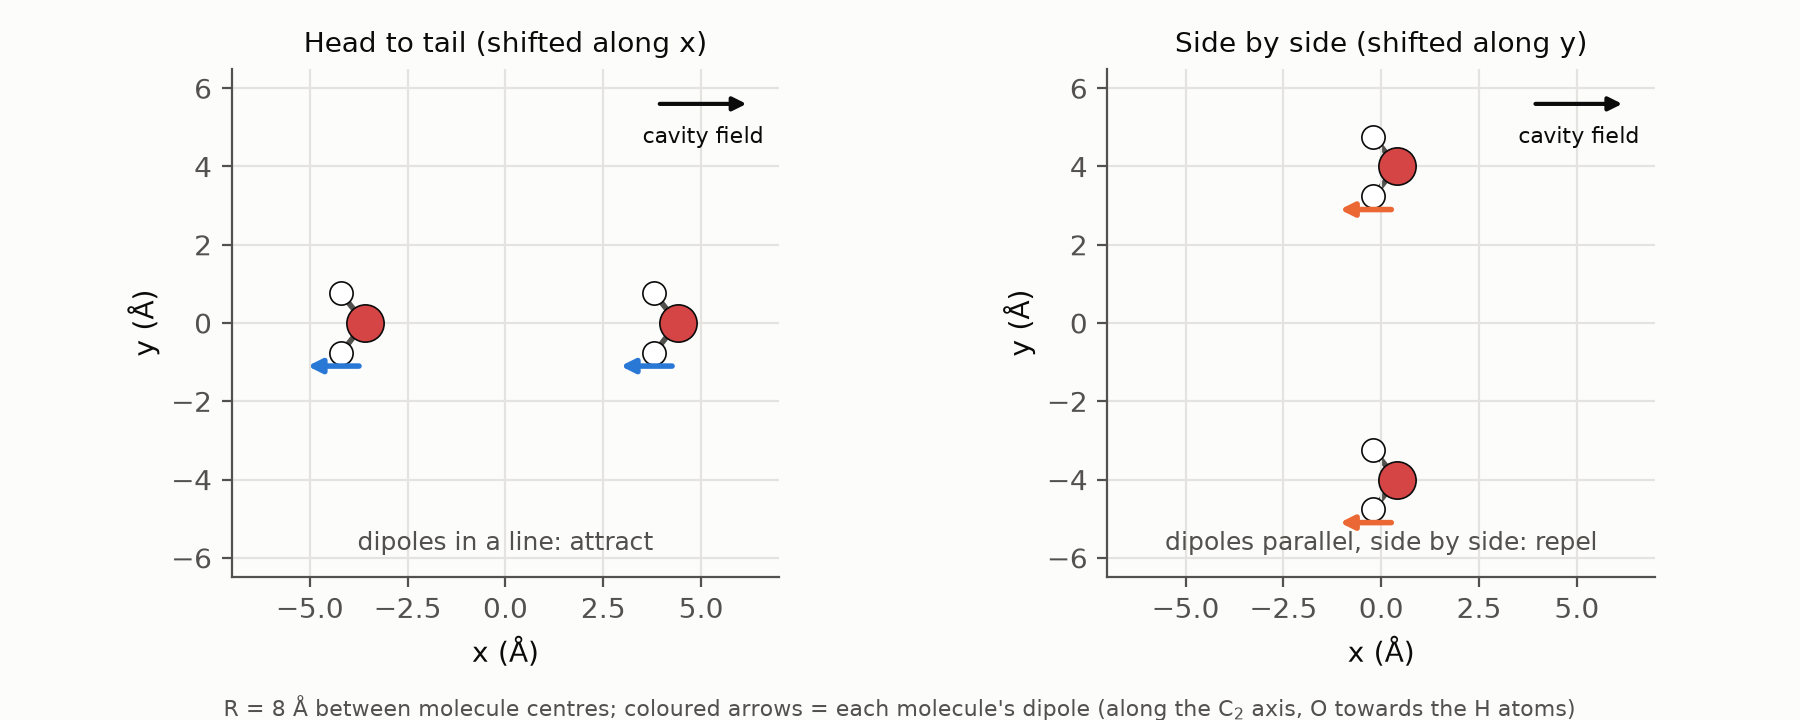
\includegraphics[width=0.95\linewidth]{h2o_N2/2026-11-18_relaxed_photon/arrangements.png}
\caption{The two starting geometries (seen from above), both with each water's dipole
along the cavity field ($x$). \texttt{scripts/make\_cluster.py} copies the single-water
geometry and shifts it by $R$. Both molecules start identical, so only the bright mode is
excited.}
\end{figure}

Settings for all runs: PySCF (LDA/cc-pVDZ), $\chi$ neglected, cavity at the bend
(1584\cm) polarized along $x$, $\lambda=0.2$, 0.5~fs steps. Two waters cost about
1.2--1.3~s per step on the laptop, so 800 steps (0.4~ps) take about 17~min and 4000 steps
(2~ps) about 1.5~h.

\section*{3. First attempt: separation scan}

Two waters head to tail at $R = 4, 6, 8, 10$~\AA, 800 steps, photon starting at $q=0$ as
in all our earlier runs.

\begin{figure}[H]
\centering
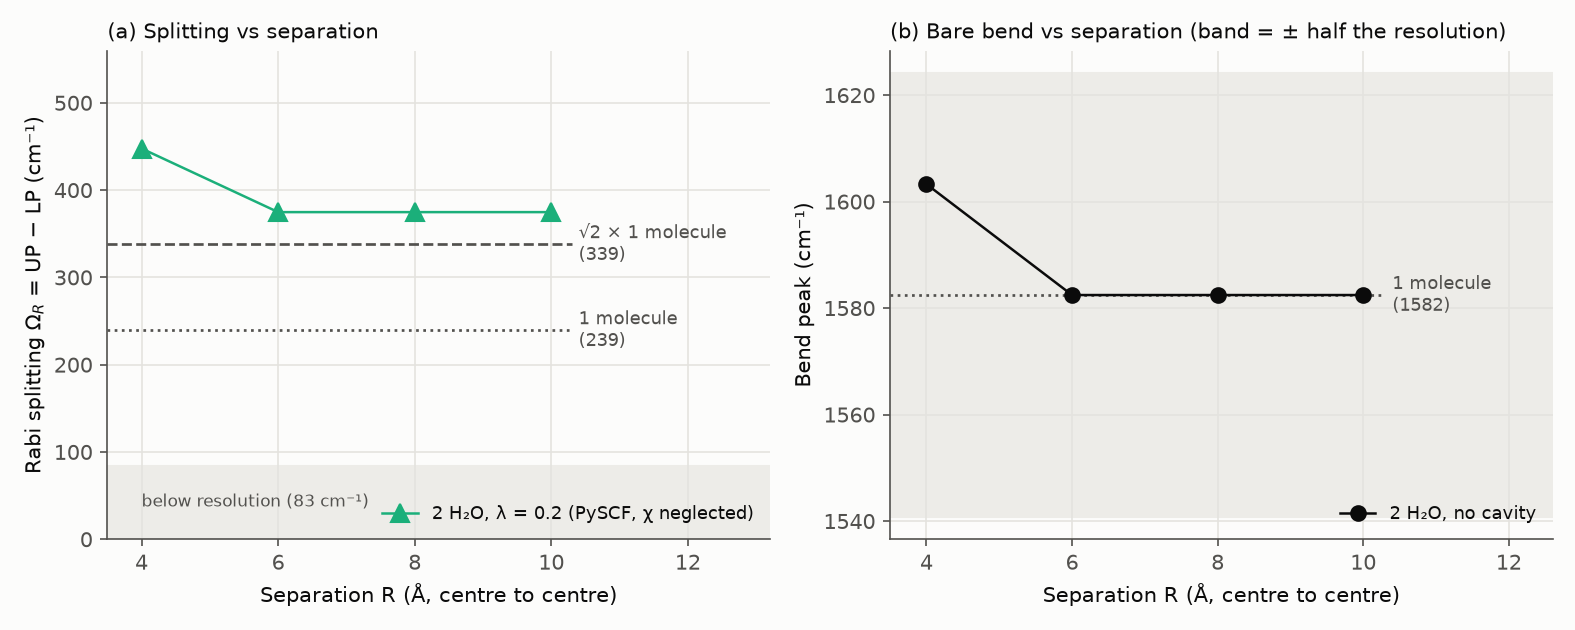
\includegraphics[width=\linewidth]{h2o_N2/2026-11-18_separation_scan/separation.png}
\caption{(a) Splitting vs separation. (b) Bend frequency without the cavity. From 6~\AA\
on, neither depends on $R$; at 4~\AA\ the molecules drift into contact (2.3~\AA) and
both change.}
\end{figure}

\textbf{What it says:} for $R\ge6$~\AA\ the waters don't feel each other (bare bend
1582\cm, same as one water), which is what we want. But the splitting is 375\cm, i.e.
1.57 times one water (239\cm), well above the expected 1.41. That pointed to something in
the setup rather than in the physics.

\section*{4. The photon start matters}

The cavity energy is $\tfrac12(\omega q - \lambda\mu)^2$, with $\mu$ the molecular dipole
along the field. Water has a permanent dipole, so at $q=0$ this is \emph{not} at its
minimum: the cavity starts with an extra energy $\tfrac12(\lambda\mu)^2$, and the photon
is ``plucked'' at $t=0$. For two waters $\mu$ doubles and this kick is four times larger.
The fix is to start the photon where the cavity energy is already at its minimum:
\[
  q_0 = \lambda\mu_x/\omega ,
\]
with $\mu_x$ the starting dipole from a PySCF single-point calculation: $q_0 = -21.46$
(one water), $-43.05$ (two, head to tail), $-42.84$ (two, side by side). This is passed to
the code with \texttt{--set qa0=$q_0$}.

\begin{figure}[H]
\centering
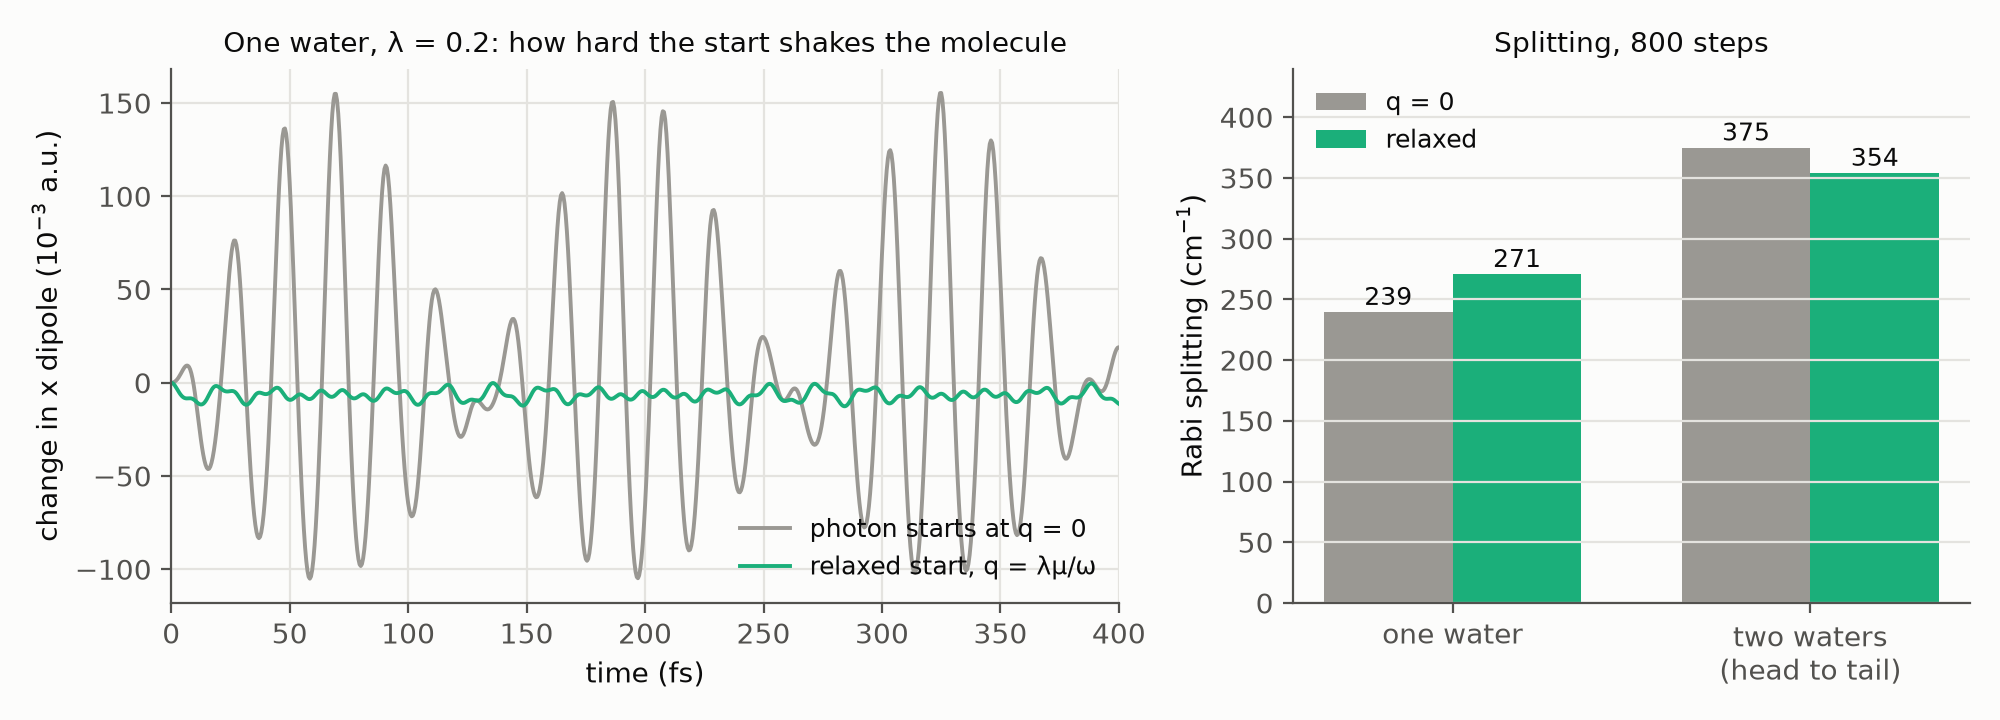
\includegraphics[width=\linewidth]{h2o_N2/2026-11-18_relaxed_photon/photon_start.png}
\caption{Left: the $x$ dipole of one water over the first 400~fs. With $q=0$ (grey) the
molecule is shaken about 23 times harder than with the relaxed start (green), and for
two waters about 32 times. Right: the splitting from each start (800 steps).}
\end{figure}

\textbf{What it says:} the $q=0$ start drives the water far from the small-oscillation
(linear) regime that the $\sqrt N$ formula assumes, and it does so more strongly for two
waters. With the relaxed start the two-water splitting drops from 375 to 354\cm, and the
one-water splitting changes from 239 to 271\cm. At 800 steps (83\cm\ resolution) the
ratio is $1.31 \pm 0.09$: now \emph{below} $\sqrt2$, but these short runs can't separate
the peaks precisely enough. So the next step was longer runs.

\textbf{Note:} all our earlier H$_2$O results (including the 2 October $\lambda$ sweep,
$\Omega_R\approx1265\lambda$) used $q=0$. Their splittings are shifted by 10--50\cm\
and should be redone with the relaxed start. CO$_2$ has no permanent dipole along the
field, so it is not affected.

\section*{5. Long runs (2 ps) and how the molecules move}

4000 steps give 8\cm\ resolution. The two-water runs were run in my own terminal (about
1.5~h each), the single water alongside.

\begin{figure}[H]
\centering
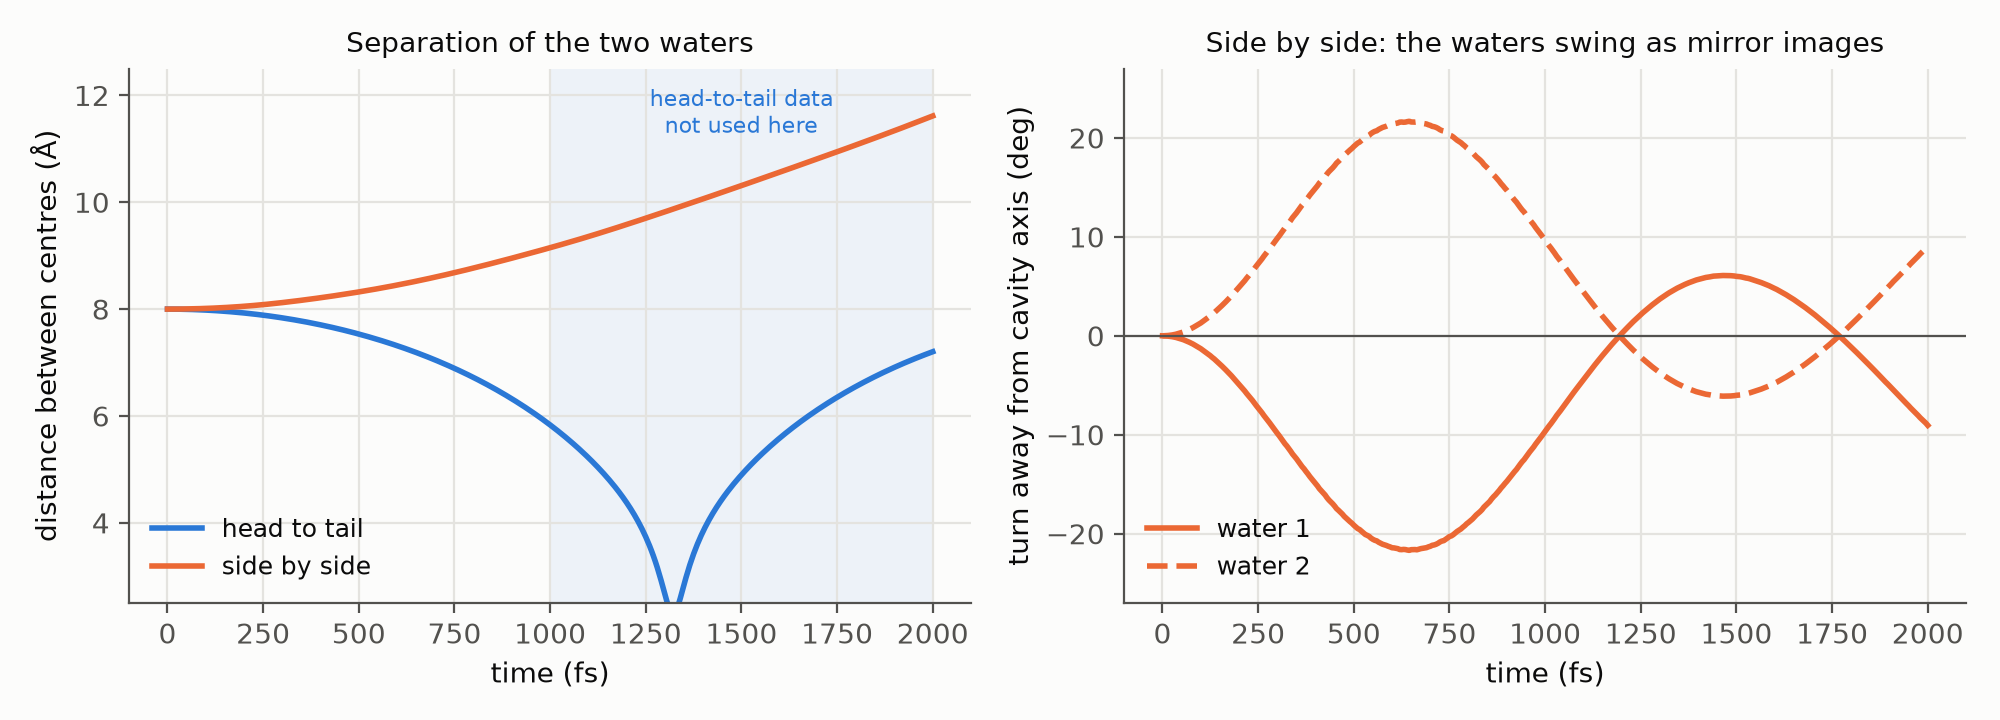
\includegraphics[width=\linewidth]{h2o_N2/2026-11-18_relaxed_photon/motion.png}
\caption{Left: distance between the two waters' centres. Head to tail (blue) they attract
and collide at 1.3~ps (closest atoms 2.3~\AA), then bounce apart; only the first 1~ps is
used. Side by side (orange) they slowly push apart, from 8.0 to 11.6~\AA. Right: side by
side, each water turns up to 22$^\circ$ away from the cavity axis and back, the two
always as mirror images.}
\end{figure}

\textbf{Why they move:} two dipoles in a line (head to tail) attract each other; two
parallel dipoles side by side repel. The cavity isn't responsible: the bare runs move the
same way. In the side-by-side case, each water also feels a small twist from the other's
field, so it swings back and forth (libration). Because the two swing in opposite
directions, their dipoles never cancel; the dipole along the field just dips by about
2\% on average.

\begin{figure}[H]
\centering
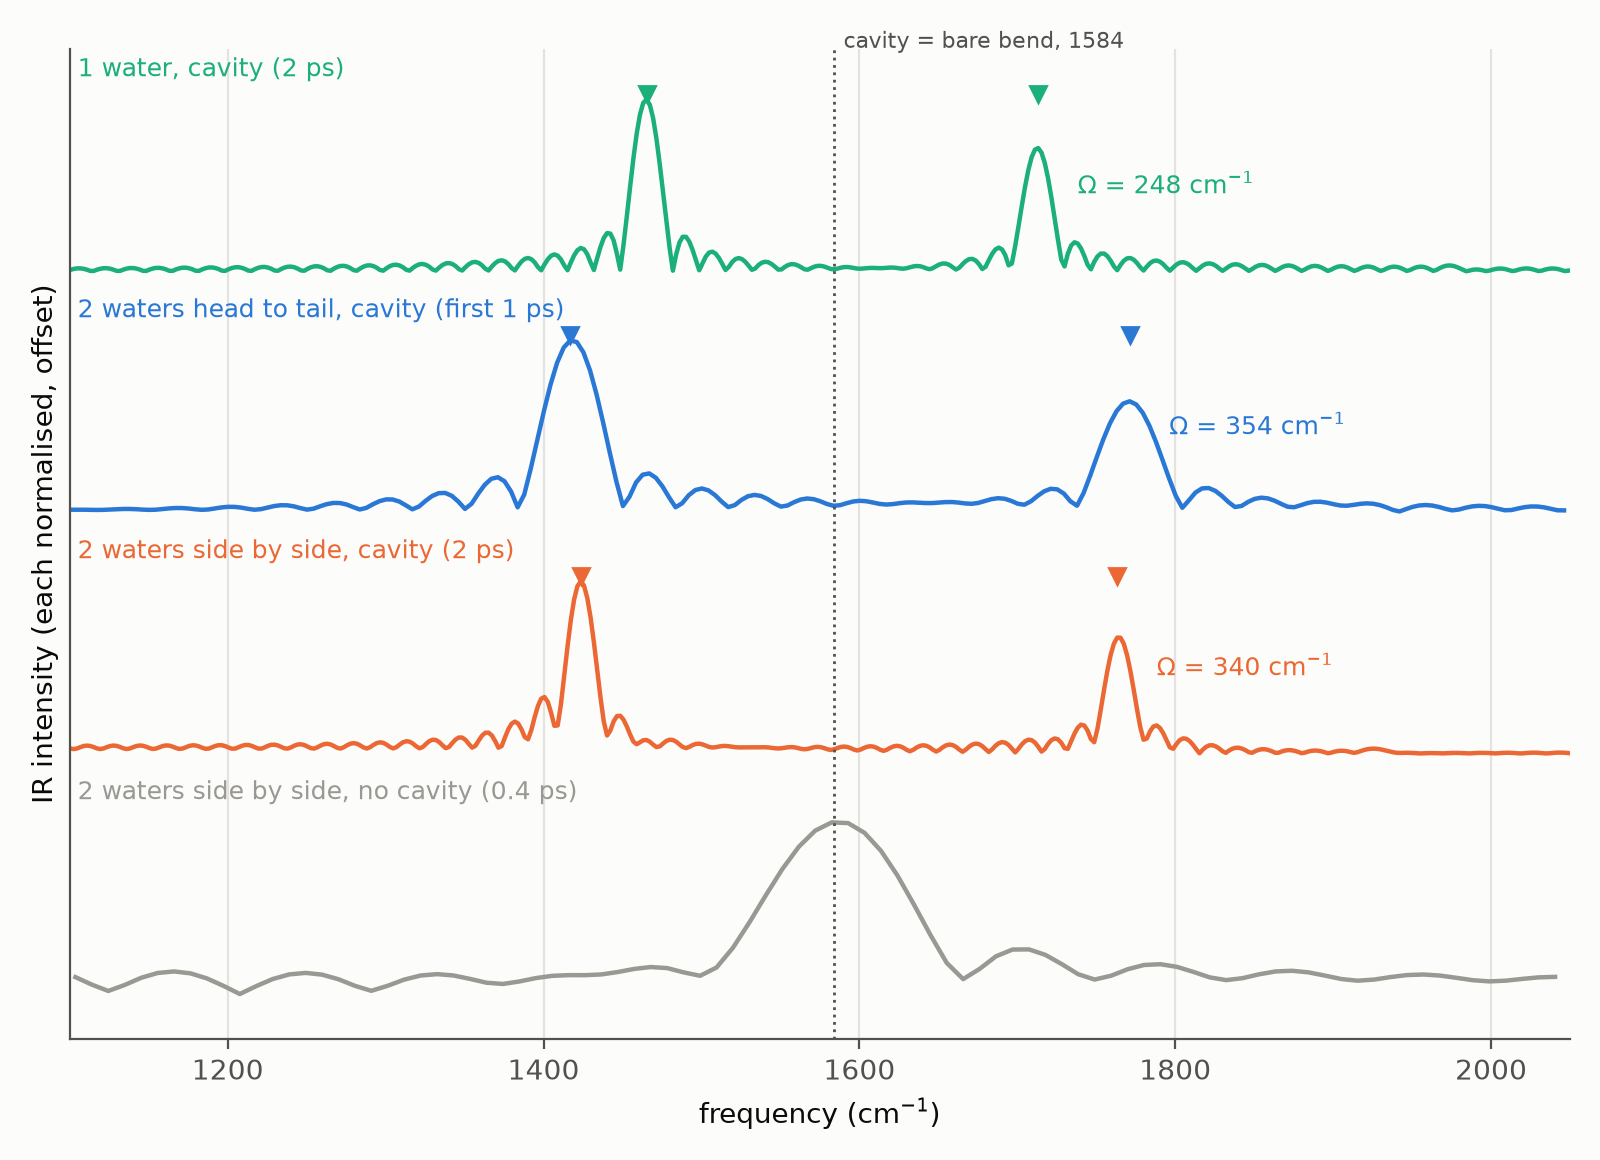
\includegraphics[width=0.85\linewidth]{h2o_N2/2026-11-18_relaxed_photon/spectra.png}
\caption{IR spectra near the bend (relaxed start, $\lambda=0.2$). Triangles mark the lower
and upper polaritons. Without the cavity (grey), the pair has a single bend peak at
1582\cm, the same as one water.}
\end{figure}

\begin{table}[H]
\centering\small
\begin{tabular}{lcccc}
\toprule
Run (relaxed start, $\lambda=0.2$) & LP & UP & $\Omega_R$ & ratio to 1 water\\
\midrule
1 water, 2~ps                         & 1465 & 1713 & 248 & --\\
1 water, first 1~ps                   & 1467 & 1713 & 246 & --\\
2 waters head to tail, first 1~ps     & 1417 & 1771 & 354 & $1.44\pm0.07$\\
2 waters side by side, 2~ps           & 1424 & 1763 & 340 & $1.37\pm0.05$\\
\bottomrule
\end{tabular}
\caption{Peak positions in cm$^{-1}$. Each ratio compares runs of equal length.
Uncertainties assume each peak position is good to about $\pm$5--7\cm\ at these lengths
(from the scatter between the two halves of the side-by-side run, 334 vs 350\cm).}
\end{table}

\textbf{What it says:} the head-to-tail ratio, 1.44, sits right on $\sqrt2$. The side-by-side
value, 1.37, is 3\% lower, still within its uncertainty. Part of the gap is the
libration: averaged over the run, each dipole's projection on the field is reduced by 2\%
($\langle\cos\theta\rangle = 0.98$, typical swing $11^\circ$), which predicts
$1.41\times0.98 = 1.39$.

\section*{6. The answer so far}

\begin{figure}[H]
\centering
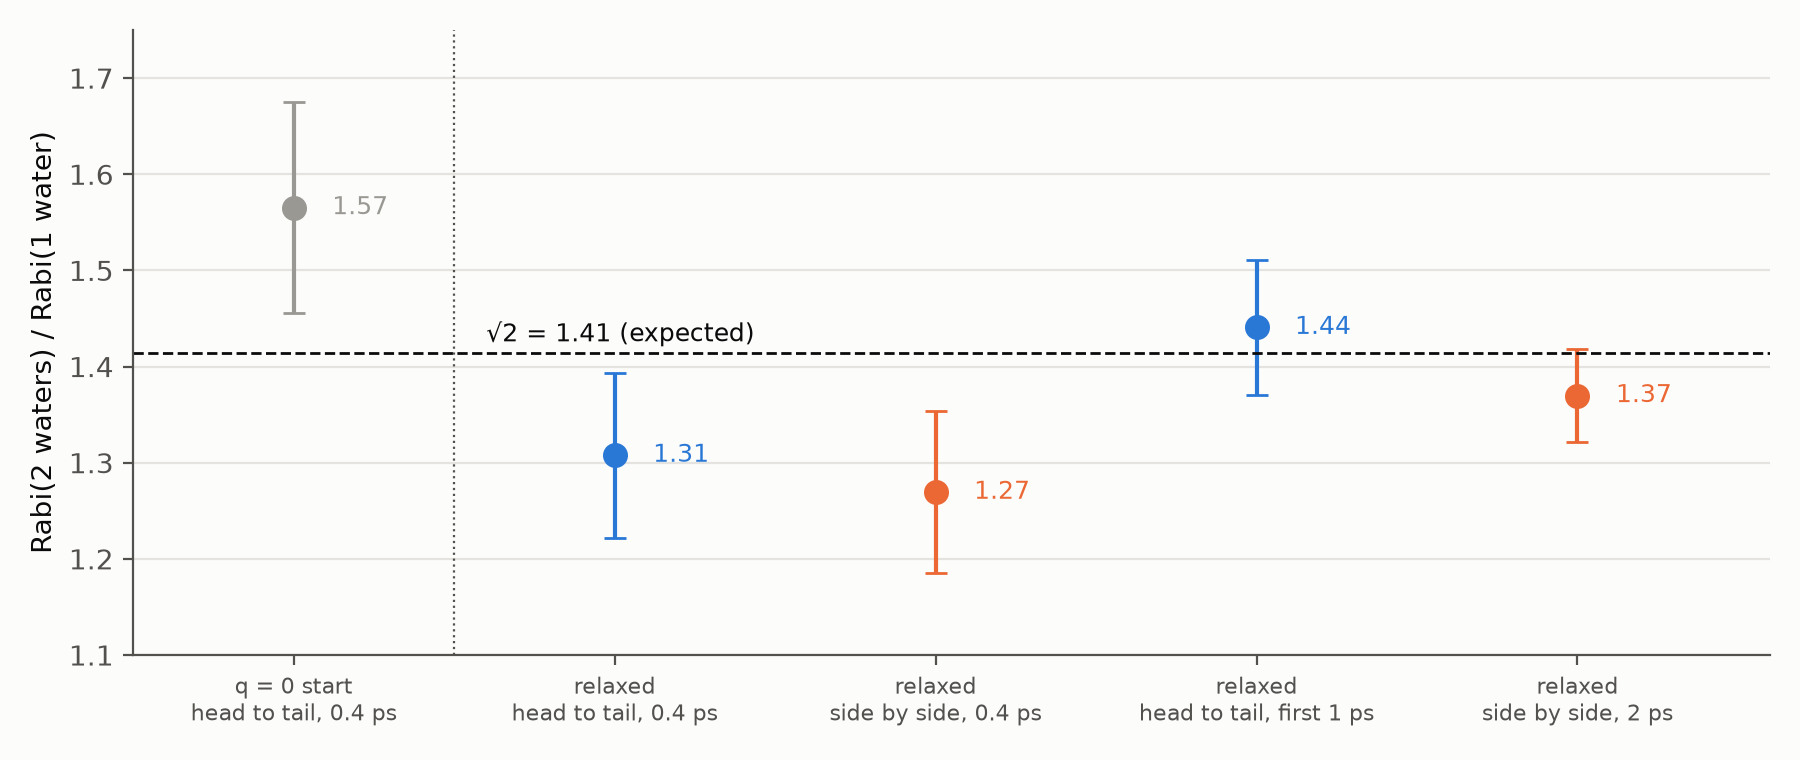
\includegraphics[width=0.9\linewidth]{h2o_N2/2026-11-18_relaxed_photon/ratio.png}
\caption{Splitting of two waters divided by one water, for every comparison made this week.
Left of the dotted line: photon starting at $q=0$. Right: relaxed start, from the short
0.4~ps runs to the long ones.}
\end{figure}

\begin{itemize}
  \item With the relaxed start, the two-water splitting is $\sqrt2$ times the one-water
        splitting, within a few percent. The cavity-mediated collective coupling works in
        our setup as it should.
  \item The 1.57 we first found came from the $q=0$ start, not from the molecules
        interacting.
  \item For more than one molecule, how the molecules move matters: they must be placed so
        that they don't run into each other, and their rotation must be tracked.
\end{itemize}

\section*{7. Checks}

\textbf{Energy conservation.} All runs conserve the total energy (including the cavity).
The long relaxed runs carry very little vibrational energy, so the automatic check, which
compares the drift to that energy, flags them; the absolute numbers are small:

\begin{table}[H]
\centering\small
\begin{tabular}{lccc}
\toprule
Long run (2 ps) & energy in motion & total-energy range & drift\\
\midrule
1 water                    & 6.5~meV  & 0.35~meV & $+0.08$~meV\\
2 waters, head to tail     & 336~meV  & 0.84~meV & $+0.12$~meV\\
2 waters, side by side     & 16.5~meV & 1.0~meV  & $-0.50$~meV\\
\bottomrule
\end{tabular}
\end{table}

(The head-to-tail run has much more motion because of the collision.)

\textbf{Correction to the 2 October report.} It said H$_2$O rotates by 49$^\circ$ when
the field is tilted by 30$^\circ$. That was the angle at the last frame. The molecule
swings back and forth, and the largest swing is 72$^\circ$. The new
\texttt{scripts/molecule\_motion.py} reports the largest swing for every run.

\section*{Next steps}

\begin{enumerate}
  \item \textbf{Relaxed start by default for water:} have \texttt{run.py} compute
        $q_0=\lambda\mu_x/\omega$ itself from a single-point dipole, so every run starts
        relaxed.
  \item \textbf{Redo the single-water $\lambda$ sweep} with the relaxed start and longer
        runs, to replace the $q=0$ numbers ($\Omega_R \approx 1265\lambda$).
  \item \textbf{Three waters side by side} (a row along $y$): check
        $\Omega_3/\Omega_1 = \sqrt3 \approx 1.73$, i.e.\ about 430\cm. Cost about
        2~s per step, so a 2~ps run takes about 2~h.
  \item \textbf{$\chi$ on for two waters:} about 5~s per step, so a 2~ps run takes about
        6~h; worth running overnight once the $\chi$-off picture is settled.
  \item \textbf{Towards liquid water:} the long-term goal needs many molecules, which needs
        a trained machine-learning model (NEP or DeepMD) for water, since PySCF is too slow.
\end{enumerate}

\section*{Questions}

\begin{enumerate}
  \item Is the relaxed photon start ($q_0=\lambda\mu/\omega$) what the group uses for polar
        molecules? Should it be the default in our runs?
  \item For multi-molecule tests, should the molecules be free to move and rotate (as
        now), or should centres or orientations be held fixed to isolate the cavity effect?
  \item For the liquid, is there a water NEP or DeepMD model in the group we can start from,
        or should we train one?
\end{enumerate}

\vfill
{\small\raggedright Data, scripts and figures: \texttt{github.com/charliew0707/VSC\_Molecular\_Dynamics}.\\
Campaigns in \texttt{scripts/campaigns/}: \texttt{h2o\_N2\_separation\_scan.sh},
\texttt{h2o\_relaxed\_photon.sh}, \texttt{h2o\_relaxed\_photon\_long.sh},
\texttt{h2o\_N2\_sidebyside.sh}.\\
Figures: \texttt{scripts/plot\_h2o\_N2\_relaxed.py}.\\
Peak table: \texttt{results/h2o\_N2/2026-11-18\_relaxed\_photon/peaks.csv}.\par}

\end{document}
